% Official contribution: https://conferences.iaea.org/event/498/contributions/43632/
% Scheduled date: 2026-10-28.
\paragraph{Abstract}
% No substantive abstract published at the time of preparation.
This talk introduces the development of Starrydata\cite{Katsura2025Starrydata}, a web-based materials property database, and shares insights from the data collection project that may be useful for similar initiatives in other research fields. Starrydata facilitates the manual extraction of numerical data from figures in scientific publications, particularly temperature-dependent thermoelectric properties. The database currently contains over 230,000 curves from more than 100,000 samples, extracted from over 66,000 figures in 17,000 scientific papers.

The largest datasets cover thermoelectric, magnetic, battery, and dielectric materials. The data collection process begins with designing a data schema and selecting target figures. Based on a list of DOIs obtained from external databases, data collection pages are automatically generated by retrieving bibliographic information from Crossref. Data collection is performed by dedicated curators, who label graph axes, trace data points, annotate sample information, and merge records corresponding to identical samples appearing in multiple figures within the same paper.

Automated data extraction methods are also under development. LLM-assisted extraction has been implemented to retrieve sample information from the experimental methods sections of scientific papers. LLMs are also used in Starrydata Auto-summary GPT, a custom GPT built on ChatGPT that summarizes the research scope, figures, samples, and experimental methods from uploaded PDF files. However, the use of LLMs is currently restricted to open-access papers published under the CC BY license. Consequently, manual data curation by dedicated curators remains the primary approach for covering a broad range of published literature.

Using the collected data, visualization tools have been developed, including composition maps, property curves, and scatter plots, to explore relationships between material compositions and thermoelectric properties. The Starrydata web system is publicly available at \url{https://starrydata.nims.go.jp}, and the entire dataset is available for download. Data collection activities are financially supported through collaborations with industrial partners interested in utilizing published research data. This talk also discusses strategies for organizing data collection teams and integrating large language models (LLMs) into the data collection workflow.
\mbox{}\par
\begin{figure}
    \centering
    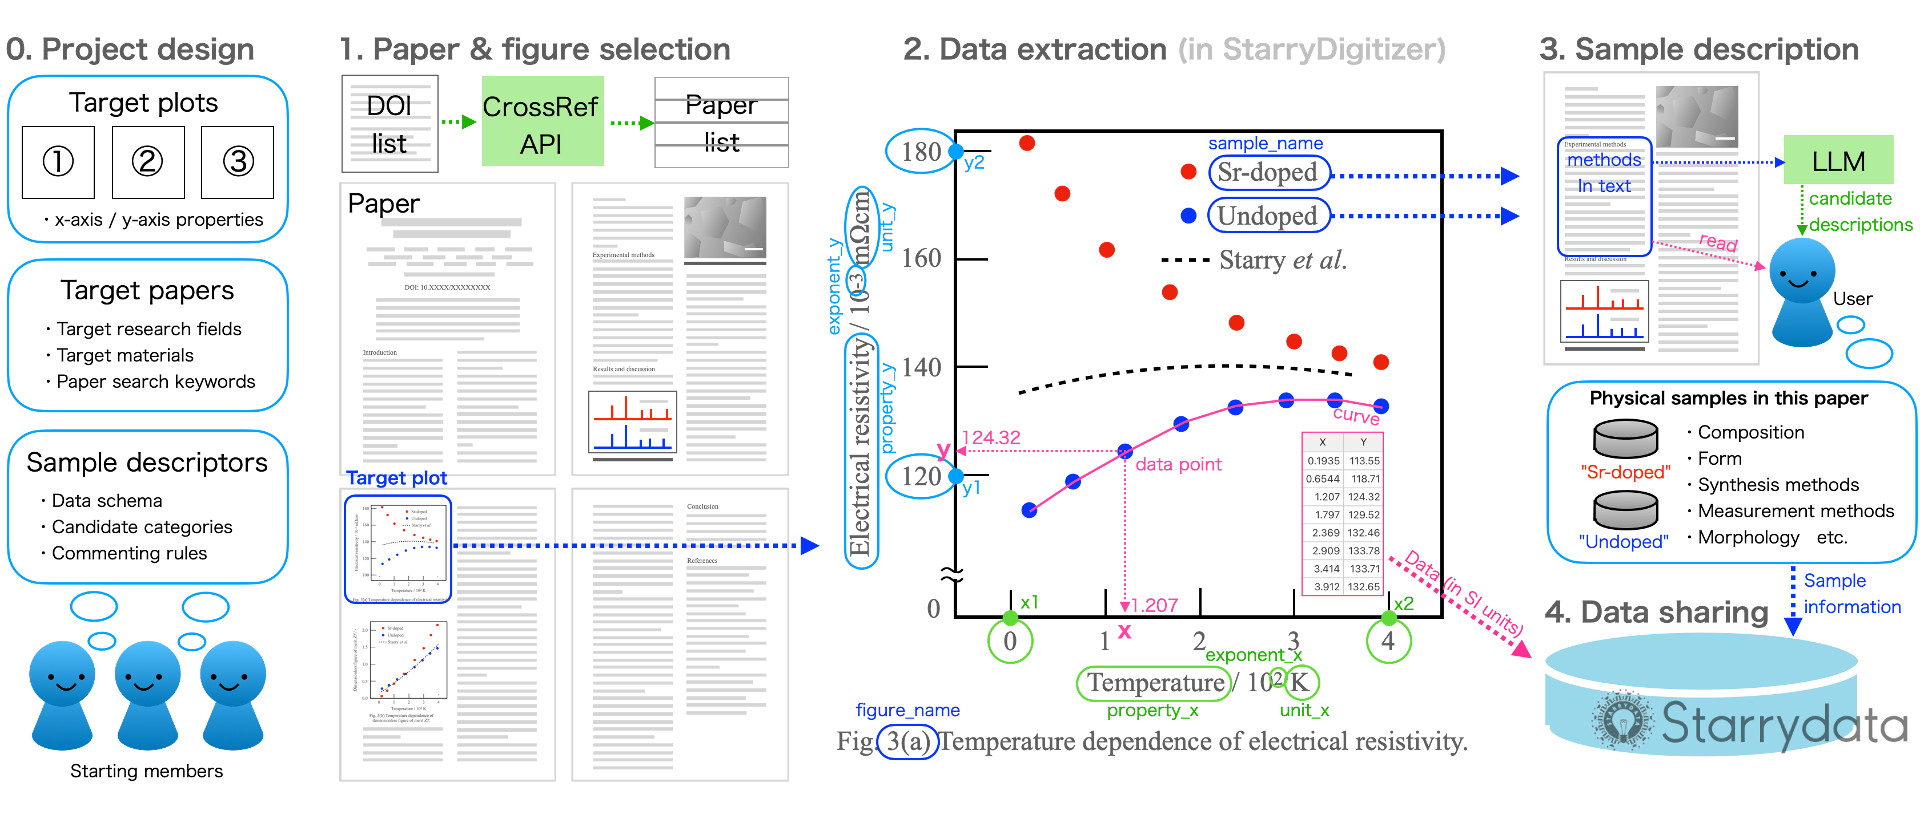
\includegraphics[width=1\linewidth]{figures/Figure1.png}
    \caption{Data collection process in Starrydata.\cite{Katsura2025Starrydata}}
    \label{fig:starrydata-collection}
\end{figure}


\paragraph{Discussion}
% Source: Webex-Summary/day1.pdf; use the meeting date, not the filename.
Yukari Katsura presented Starrydata's collection of numerical materials data from published figures, with sample metadata and links to source articles. The presentation described curation tools, manual digitisation and assisted extraction. Discussion covered overlapping traces, figure quality, digitisation errors and the limits of automation. Language models were considered for metadata preparation with human checking. Participants also discussed sustaining curation, discovering available properties and connecting experimental records to other materials resources. The examples offered experience relevant to literature-based nuclear data collection, while differing sample definitions and data models complicate direct integration.
